\chapter{Essential Concepts and Tools} \label{tools}
Before delving into the discussion of the theorem, let us recall some basic notions that will be essential for what we will discuss later. 
In particular, having a clear understanding of this information will be crucial to ensuring a thorough comprehension of the assumptions considered and the demonstration techniques employed.

First of all, to begin familiarizing ourselves with the notation, let us review the classification of partial differential equations of order $k$, and consequently the associated operators, with a summary table.
\vspace{5mm}
\begin{center}
\renewcommand{\arraystretch}{2}
\begin{tabular}{l l} 
\hline \hline
 Linear & $\sum_{|\alpha |\leq k} a_\alpha \, D^\alpha u = f$ \\ 
 \hline
 \vspace{-2mm}
 Quasi-linear & $\sum_{|\alpha |= k} a_\alpha (x,D^\beta u) \, D^\alpha u +  a_0(x,D^\beta u)= f,$\\ 
 & $\quad |\beta |<k $ \\
 \hline
 Fully nonlinear & $F(x,D^\alpha u)=0, \quad |\alpha | \leq k$ \\ 
 \hline
 In normal form & $D_{t}^k u = G(x,t, D^\alpha_x D^j_t u), \quad |\alpha |+j \leq k, \, j < k$ \\ 
 \hline \hline
\end{tabular}
\end{center}
\vspace{5mm}
\begin{remark}
From here on, we will not always pay particular attention to the regularity assumptions on the data of the equations ($f,a_\alpha,F,G$, and others), since for our purposes it is enough that the statements hold in the case where everything is assumed to be analytic (with a certain radius of convergence). The same applies to the data and the surfaces of the associated Cauchy problems. In any case, when not specified, the regularity can be considered as at least $C^1$.
\end{remark}
\begin{remark}
In the case of an equation in normal form, the variables are split between space $x\in \mathbb{R}^{n-1}$ and time $t$, for a reason that will become clear by the end of this chapter.
\end{remark}
We already anticipate that, later on, we will assume the coefficients and functions defining the equations to be very regular, specifically analytic (i.e., locally expandable in power series).
\newpage
In light of what has been said so far, we realize that there are already some aspects that would be important to focus on. 
But to be more organized, let us summarize our topics of interest in four points, which reflect the structure of this chapter:
\begin{enumerate}
\item \textbf{Characteristic surfaces}: that is, those surfaces in $\mathbb{R}^n$ that are closely related to the form of the equation in observation and can pose problems when deciding to assign Cauchy data on them;
\item \textbf{Method of characteristics}: in the case of first-order, possibly nonlinear, equations, a PDE can be viewed as a system of ODEs dependent on a parameter;
\item \textbf{Cauchy problems}: the only type of problem we will deal with;
\item \textbf{Power series}: these form the foundation of the concept of an analytic function (and holomorphic in the case of complex numbers), which is the only type of function we will seek as a solution.
\end{enumerate}

\section{Characteristic Surfaces} \label{supcar}
In this first section, we introduce the concept of a characteristic surface in the simplest cases, to fully understand its meaning. Let us begin by considering the simplest situation of all, namely that of a \textbf{linear} equation. 
Such an equation is uniquely determined by the forcing term we called $f$ and by a linear differential operator $L=\sum_{|\alpha |\leq k} a_\alpha \, D^\alpha$. Let us focus on the latter and provide three definitions.

\begin{definition}
The characteristic form of $L$ is 
$$\chi_L(x,\xi)=\sum_{|\alpha |= k} a_\alpha(x) \, \xi^\alpha \text{ where } {x,\xi \in \mathbb{R}^n}.$$
\end{definition}

\begin{definition}
The characteristic variety of $L$ at $x$ is the set $$\text{char}_x (L)= \{ \xi \neq 0 : \chi_L(x,\xi)=0 \}.$$
\end{definition}

\begin{definition} \label{supcarlin}
$\Gamma$ is a characteristic surface for $L$ at $x$ if $\boldsymbol{\nu}(x) \in\text{char}_x (L)$, where $\boldsymbol{\nu}(x)$ denotes the unit normal to $\Gamma$ at $x$.
\end{definition}

Let us now investigate the meaning of these definitions:
\begin{itemize}
\item First of all, notice that when $\xi \in \text{char}_x (L)$, it is as if the operator were not "properly" of order $k$ in the direction $\xi$.
\item Additionally, in the case of a first-order operator ($k=1$), a surface $\Gamma$ is characteristic when $A=(a_1,\ldots ,a_n)$ is tangent to $\Gamma$ point by point (i.e., for every $x\in \Gamma$).
\item It is possible to show that a characteristic surface "carries more information" when Cauchy conditions are assigned on it. In fact, given the normal derivatives $D^j_\nu u \,(j<k)$ of a function $u$ that we want to satisfy the equation, if $\Gamma$ is non-characteristic at every point, it is possible to calculate all the partial derivatives of $u$ on $\Gamma$.
\end{itemize}
\newpage
Especially the last consideration, due to the lack of rigor, may be confusing at first reading. However, there exists a theorem that explicitly shows this result in the case of quasi-linear equations and can be found together with the proof in \cite[cap.4.6]{Evans}.

\noindent\rule[0.5ex]{\linewidth}{0.2pt}
Given that we aim to prove a theorem that will turn out to be very general, we note that, unfortunately, linear equations will not be sufficient to solve all our problems. For this reason, we want to immediately generalize the concept of a non-characteristic surface to the \textbf{quasi-linear} case, even though we still remain in the first-order equation scenario. Now, suppose we have the Cauchy problem
\begin{equation}
\begin{cases}
\sum a_j(x,u)D_{x_j} u = b(x,u)\\
u = \phi \text{ on } \Gamma
\end{cases}
\end{equation}
and that $\Gamma$ has a local parametrization near $x_0\in \Gamma$ given by the function $\gamma (s): \mathbb{R}^{n-1}\rightarrow \mathbb{R}^n$, we provide the following generalization, clearly inspired by the case of first-order linear operators.
\begin{definition}
$\Gamma$ is non-characteristic at $x_0=\gamma (s_0)$ if\\
\begin{equation*}
\det
\underbrace{
\left[
\begin{matrix}
D_{s_1}\gamma_1 & \cdots & D_{s_{n-1}}\gamma_1 \\
\vdots &  & \vdots \\
D_{s_1}\gamma_n & \cdots & D_{s_{n-1}}\gamma_n \\
\end{matrix}\;\right|}_{\text{span of the tangent plane}} \,
\left.
\begin{matrix}
a_1(\gamma, \phi(\gamma))\\
\vdots\\
a_n(\gamma, \phi(\gamma))\\
\end{matrix}\right] (s_0) \neq 0.
\end{equation*}
\end{definition}
Now it is time to use these definitions to draw some useful conclusions.


\newpage
\section{Method of Characteristics}\label{metodocar}
Let us consider an application of the notion of non-characteristic surface: the method of characteristics for first-order PDEs. 
This is a method for finding solutions to equations, possibly even fully nonlinear, which is based on the idea of transforming the problem into a system of ODEs that is equivalent.

We start directly from the case of a quasi-linear equation and consider again the corresponding Cauchy problem with data assigned on some surface $\Gamma$. We want to show that this problem is \textbf{equivalent} to another problem for a system of ODEs.
\begin{align} 
\label{edpquasilin}
\text{PDE : }&
\begin{cases}
\sum a_j(x,u)D_{x_j} u = b(x,u)\\
u = \phi \text{ on } \Gamma
\end{cases} \\ 
\label{sisedo}
\text{ODE : }&
\begin{cases}
D_t \, x = A(x,y) \; \\ 
D_t \, y = b(x,y)\\ 
x(0)=x_0, \; y(0) = \phi (x_0) \quad \forall x_0 \in \Gamma
\end{cases} 
\end{align}
where $y = u(x)$ and $A(x,y)=(a_1(x,y),\ldots ,a_n(x,y))$.
\begin{remark}
It is important to highlight three aspects:
\begin{itemize}
\item the solutions $x$ are called \textbf{characteristic curves};
\item the second problem is parametric with respect to $x_0$, so the entire solution for $u$ will be given by the union over all $x_0\in \Gamma$ of all the $y$ along the curves $x$;
\item the case of linear equations is immediate to derive from what has been stated above, simply by assuming that the coefficients $a_j$ depend only on $x$ and that $b$ is of the form $b(x,u)=f(x)-c(x)u$.
\end{itemize}
\end{remark}
Without providing a precise statement, let us proceed with a reasoning that is still rigorous, which can be considered a proof of the equivalence.
\begin{proof}
In both directions, a simple derivation of a composed function:
\begin{enumerate}
\item Suppose we know, for every $x_0$, $y(t)$ and $x(t)$ that solve the problem \eqref{sisedo}. Then for every $x_0$ it holds that:
$$b(x,y) = D_t y = \sum D_{x_j} y \; D_t x_j = \sum a_j(x,y) D_{x_j} y.$$
From which it follows that the function $u(x)$ that has a graph given by the union of all the curves $(x(t),y(t))$ solves the problem \eqref{edpquasilin}.
\item Now assume instead that we know $u$, a solution of \eqref{edpquasilin}. We find $x$ by solving $\forall j$:
\begin{equation*} \label{sys}
D_t \, x_j = a_j(x,y), \quad x_j(0)=(x_0)_j 
\end{equation*}
We define $y(t)=u(x(t))$ and finally, we use the same reasoning as before to conclude that $y$ satisfies the equation of the ODE system:
$$D_t y = \sum D_{x_j} u \; D_t x_j = \sum  a_j(x,y)D_{x_j} u = b(x,y).$$
\qedhere
\end{enumerate}
\end{proof}
At this point, one might wonder where the idea of verifying the equivalence with that specific system of ODEs arises. The answer to this question is interesting because it encompasses the geometric meaning of this method. In fact, recalling that the normal vector to the graph of a function $u$ is proportional to the vector $(\nabla u , -1)$, we can state that the equation \eqref{edpquasilin} tells us that the following vector field must be \textbf{tangent} to the graph of $u$.
$$(a_1(x,u(x)),\, \ldots ,\, a_n(x,u(x)),\, b(x,u(x)))=(A(x,u(x)),\, b(x,u(x)))$$

\noindent\rule[0.5ex]{\linewidth}{0.2pt}

Understanding this last aspect begins to outline the role of the characteristic property of a surface. \\
Now let us see a theorem to concretize this intuition.
\begin{theorem}\label{teoescar}
\hpth{
\text{Problem \eqref{edpquasilin} } \\ 
a_j, \, b, \, \phi , \, \Gamma \in C^1\\ 
\Gamma \text{ is non-characteristic}
}{
\exists ! \text{ solution } C^1 \text{ in a neighborhood of } \Gamma
}
\end{theorem}
The complete and detailed proof can be found in \cite[cap.1]{Folland}; here we only mention the fundamental ideas. The uniqueness follows simply from the fact that the graph of the solution $u$ can be seen as the union of the curves $(x(t),y(t))$, which do not intersect if one takes a sufficiently small neighborhood of $\Gamma$. To prove existence, the representation of the equation as a parametric set of systems of ODEs is used to carry out the following steps:
\begin{enumerate}
\item apply the local existence and uniqueness theorem for ODEs;
\item prove the invertibility of $x(s,t)$, where $s$ is an auxiliary variable related to the local parameterization of $\Gamma$, thanks to the fact that it is non-characteristic;
\item thus define the solution $u(x)$ easily following the same idea from point 1 of the last proof made;
\item verify with the derivative of a composed function that $u$ is a solution of the equation.
\end{enumerate}
Both the definition of characteristic surface and the method of characteristics can be generalized to the case of a generic first-order equation. Moreover, there is also a generalization of theorem \ref{teoescar} for the fully nonlinear case, identical in both spirit and substance to the quasi-linear case.
We will not address this topic in detail, as it does not add anything at a qualitative level of understanding of the subject and will not be useful in the subsequent discussion. For further reading, one can refer to \cite[cap.1]{Folland} and \cite[cap.3]{Evans}.

However, the notion of non-characteristic surface is not sufficient for our purposes, and in the next paragraph, we want to extend it to the most general possible case: fully nonlinear equations of any order.

\newpage
\section{Cauchy Problems} \label{pb}

So far, we have only seen the simplest case of a Cauchy problem, namely that for a first-order equation, where it is necessary to assign only the value of the function on a surface. For an equation of any order, this information is not sufficient to uniquely determine the solution; typically, what is done is to also assign the \textbf{normal derivatives} of the solution $D^j_\nu u$ with $j<k=$ order of the equation.

\noindent\rule[0.5ex]{\linewidth}{0.2pt}

In light of what has been stated in the previous two paragraphs, we have already inferred that the notion of non-characteristic surface is useful for identifying those surfaces on which we want to assign Cauchy conditions in such a way as to have some guarantee of the existence of the solution in the neighborhood of the surface. We will now focus on understanding what is meant by a characteristic surface in the most general case we can imagine, following the simplest and most direct approach possible, as it does not require particular proofs.
Let us consider the Cauchy problem:
\begin{equation}
\begin{cases}
F^*(x,D^\alpha u^*)=0 & |\alpha | \leq k, \, F^*\\
D^j_\nu u^* = \phi_j^* & \text{on } \Gamma^* \text{ for } j<k 
\end{cases}
\end{equation}

Regardless of the form of the equation, it is possible to modify this problem in such a way as to locally flatten the boundary of the surface with respect to a variable. To achieve this result, a simple change of coordinates $\Phi$, defined via $\gamma^*$ (local parameterization of $\Gamma^*$), is sufficient:
$$\Phi (x) = 
\left( \begin{matrix}[ccc|c]
x_1 & \cdots & x_{n-1} & x_n-\gamma^* (x_1,\ldots , x_{n-1})
\end{matrix}\right).$$
\begin{figure}[H]
\centering
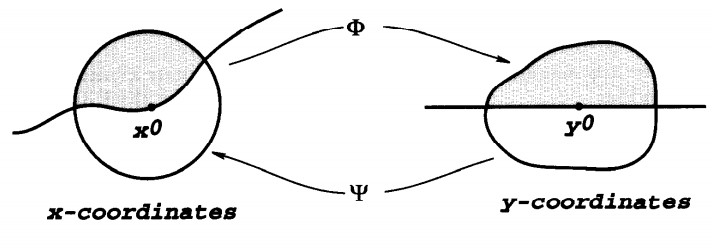
\includegraphics[scale=.5]{flatb}
\caption{Image from \cite[cap.8]{Evans}}
\end{figure}
\begin{remark}
Note that $\Phi$ preserves any analyticity of the surface $\Gamma^*$.
\end{remark}

This transformation helps us understand how it is possible to choose to consider one variable as "privileged." From now on, this variable will be referred to as "time," and we will denote it with the letter $t$. To be more precise, we rename the variables as follows:
\begin{align*}
t & \leftarrow x_n \\ 
x & \leftarrow (x_1,\ldots , x_{n-1})
\end{align*}

\newpage
Furthermore, we introduce some notation that will be useful later:
\begin{itemize}
\item we denote $\Gamma_0 = \{t=0\}$;
\item we indicate the derivatives as follows: $D^\alpha_x D^j_t u$.
\end{itemize}
We conclude that thanks to the transformation $\Phi$, we obtain the new problem:
\begin{equation}\label{gamma0prob}
\begin{cases}
F(x,t, D^\alpha_x D^j_t u)=0 & |\alpha | +j \leq k\\
D^j_t u (x,0)= \phi_j(x) & \text{for } j<k 
\end{cases}
\end{equation}
where $u^*=u(\Phi)$.

\noindent\rule[0.5ex]{\linewidth}{0.2pt}

\begin{definition}
$\Gamma^*$ (or $\Gamma_0$) is non-characteristic if the equation on $\Gamma_0$ can be rewritten in \textbf{normal form} with respect to $t$, that is, if the problem \eqref{gamma0prob} can be rewritten as follows:
\begin{equation*}
\begin{cases}
D_{t}^k u = G(x,t, D^\alpha_x D^j_t u) & |\alpha |+ j \leq k, \, j<k \\ 
D_t^ju = \phi_j & \text{ on } \Gamma_0, \, j<k
\end{cases} \\
\end{equation*}
\end{definition}

To make this definition more concrete, sufficient conditions, and possibly also necessary ones, are often sought so that the equation can be rewritten in normal form, as we did in the paragraph \ref{supcar} for the simplest cases and as was done in \cite{Evans} and \cite{Folland}.
Let us therefore examine what this involves, distinguishing the various cases and assuming we have already placed ourselves in the situation \eqref{gamma0prob}:
\begin{itemize}
\item linear and quasi-linear: it is required that $a_{(0,\ldots ,0,k)} \neq 0$ on $\Gamma_0$;
\item fully nonlinear: it is required that the hypotheses of the implicit function theorem (also known as Dini's theorem) hold for $F$, that is, $D_{(D^k_t u)} F \neq 0$ on $\Gamma_0$.
\end{itemize}

\begin{remark}
Staying within the assumption that the surface is $\Gamma_0$, starting from these considerations, it is easy to see how the new definition of non-characteristic surface is consistent with the definitions in paragraph \ref{supcar}.
\end{remark}

Finally, we recall that the notion of characteristic surface must guarantee us the ability to calculate all the partial derivatives of the solution on the surface. For this reason, the setup of this construction is partially inspired by \cite[cap.3]{Evans}, where the proof of this property is presented in two steps:
\begin{enumerate}
\item first, we reason assuming to be on $\Gamma_0$;
\item thanks to the transformation $\Phi$, we obtain the property for a generic $\Gamma^*$.
\end{enumerate}

\newpage
\section{Power Series}\label{powerseries}
Assuming the theory of holomorphic functions is known, and consequently also the basic theory of analytic (real) functions, in this paragraph we want to discover, or better understand, only a few very specific tools that will allow us to prove the TCK.

Let’s begin by studying a power series expansion of a function that we must not forget.
\begin{definition}
The majorant function is given by $$\mathcal{M}_{Cr}(x)=\frac{Cr}{r-(x_1+\ldots +x_n)}$$
\end{definition}
Using the multinomial theorem, we demonstrate that this function can be developed into a power series for $|x|<r/n$, deriving the expression for the coefficients $c_\alpha$:
\begin{align*}
\mathcal{M}_{Cr}(x) &= \frac{Cr}{r-(x_1+\ldots +x_n)} = C \sum\limits_{j=0}^\infty \left(\frac{x_1+\ldots +x_n}{r}\right)^j  \\ 
&= C \sum\limits_{j=0}^\infty \frac{1}{r^j} \sum\limits_\alpha  \binom{|\alpha |}{\alpha } x^\alpha = \sum\limits_\alpha 
\underbrace{C \frac{|\alpha |!}{\alpha ! \, r^{|\alpha |}}}_{c_\alpha} \, x^\alpha .
\end{align*}

From this result, we want to state two theorems, which constitute the backbone of the so-called majorant method, first devised by Cauchy, and which justify the terminology introduced earlier.

\begin{theorem}[Utility of the Majorant]\label{theomaj}
\hpth{
g_\alpha \geq |f_\alpha|\\
\sum g_\alpha x^\alpha \text{ has radius of convergence } R
}{
\sum f_\alpha x^\alpha \text{ has radius at least } R
}
\end{theorem}

\begin{theorem}[Construction of the Majorant]\label{constmaj}
\hpth{
\sum f_\alpha x^\alpha \text{ has radius } R
}{
\exists \, r<R, \, C>0 : \, |f_\alpha | \leq C \frac{|\alpha |!}{\alpha ! \, r^{|\alpha |}}
}
\end{theorem}

\begin{proof}
It is sufficient to note that taking $C \geq |f_\alpha r^{|\alpha |}|$ immediately implies that
$$|f_\alpha | \leq C \frac{1}{r^{|\alpha |}} \leq C \frac{|\alpha |!}{\alpha ! \, r^{|\alpha |}}.$$
\end{proof}

In the case where the hypotheses of theorem \ref{theomaj} hold, we will write:  $\sum g_\alpha x^\alpha \gg \sum f_\alpha x^\alpha$.

\begin{remark}
The same theorems continue to hold in the case of complex numbers.
\end{remark}

We conclude the paragraph and the chapter with some properties for manipulating power series. 
First of all, let’s deal with the operation of composition.
\begin{theorem}
\hpthml{
y: \mathbb{R}^n \rightarrow \mathbb{R}^m \text{ such that } y(x) = \sum y_\alpha (x-x_0)^\alpha \text{ in a neighborhood of } x_0\\
g: \mathbb{R}^m \rightarrow \mathbb{R}^d \text{ such that } g(y) = \sum g_\beta (y-y_0)^\beta \text{ in a neighborhood of } y_0=y(x_0)\\
f = g \circ y
}{
\exists \; f_\gamma = P_\gamma (g_\beta, \, y_\alpha \text{ with } \alpha_i \leq \gamma_i) \text{ set of coefficients such that } \\ 
- \; P_\gamma \text{ are polynomials with non-negative coefficients }\\
-  \; f (x) = \sum f_\gamma (x-x_0)^\gamma
}
\end{theorem}
\begin{remark}
The form of the polynomials $P_\gamma$ does not depend on $g$ and $y$.
\end{remark}
\begin{proof}
It is easy to convince oneself of this by explicitly writing the composition of the two series, especially regarding the fact that the coefficient $f_\gamma$ depends only on the $y_\alpha$ such that $\alpha_i \leq \gamma_i$.
\end{proof}

Assuming, for simplicity, that we are at the origin and recovering the notation $(x,t)$ from the previous paragraph, we state a simple rewriting of this theorem.
\begin{theorem}[Composition]\label{composition}
\hpthml{
y: \mathbb{R}^n \rightarrow \mathbb{R}^m \text{ such that } y(x,t) = \sum y_{\alpha j} \; x^\alpha t^j \text{ in a neighborhood of the origin}\\
g: \mathbb{R}^m \rightarrow \mathbb{R}^d \text{ such that } g(y) = \sum g_\beta \; y^\beta \text{ in a neighborhood of the origin }\\
f = g \circ y
}{
\exists \; f_{\gamma k} = P_{\gamma k} (g_\beta, \, y_{\alpha j} \text{ with } j \leq i) \text{ set of coefficients such that } \\ 
- \; P_{\gamma k} \text{ are polynomials with non-negative coefficients }\\
-  \; f (x,t) = \sum f_{\gamma k} \; x^\gamma t^k \label{power_series} \numberthis
}
\end{theorem}

Another way to obtain a series of the type in \eqref{power_series} is to use differentiation with respect to any variable $x_i$. Let’s see it with the following theorem.
\begin{theorem}[Differentiation]\label{derivative}
\hpth{
y: \mathbb{R}^d \rightarrow \mathbb{R}^m \text{ such that } y(x,t) = \sum y_{\alpha j} \; x^\alpha t^j \text{ in a neighborhood of the origin}\\
}{
f=D_{x_i}y \text{ is a power series as in \eqref{power_series} in a neighborhood of the origin}
}
\end{theorem}
\begin{proof} By differentiating term by term, we obtain
$$ D_{x_i} \sum y_{\alpha j} \; x^\alpha t^j = \sum  \underbrace{(\alpha_j+1) \, y_{(\alpha+e_i)j}}_{f_{\alpha j}} \; x^\alpha t^j. \; \footnotemark$$ \footnotetext{$e_i$ is the multi-index that equals 1 at its $i$-th component and 0 otherwise}
It is immediate to verify the other properties of $f_{\alpha j}$.
\end{proof}

Finally, we are interested in seeing what happens when we multiply two series like in \eqref{power_series}, obtained using one of the methods (theorems \ref{composition} and \ref{derivative}), starting from the same series $y$.
\begin{theorem}\label{product}
\hpth{
f^1, f^2 \text{ are series constructed with one of the two methods using the same } y
}{
f = f^1 f^2 \text{ is a power series as in \eqref{power_series} in a neighborhood of the origin }
}
\end{theorem}

\begin{remark}
The mixed case is also admissible, where $f^1$ is obtained with a composition and $f^2$ with a differentiation, and that is exactly what we will use.
\end{remark}

\begin{proof} By deriving the expression for the coefficients of $f$, we obtain that
$$f_{\gamma k} = \sum_{\substack{\omega+\theta=\gamma \\ l+h=k}} f^1_{\omega l}\;  f^2_{\theta h}\, .$$
Consequently, $f_{\gamma k}$ will certainly be a polynomial with non-negative coefficients, since this property is preserved under sums and products. Moreover, noting that $l,\, h \leq k$, it can be shown that each individual polynomial $f_{\gamma k}$ inherits the property from $f^1_{\omega l}$ and $f^2_{\theta h}$, meaning that it depends only on the $y_{\alpha j}$ where $j \leq k$.
\end{proof}
